\newsection
\subsection{Vision}
\label{sec:vision}
\sectionauthors{Shyamal Buch, Drew A. Hudson, Frieda Rong, Alex Tamkin, Xikun Zhang, Bohan Wu, Ehsan Adeli, Stefano Ermon, Ranjay Krishna, Juan Carlos Niebles, Jiajun Wu, Li Fei-Fei}

\begin{figure}[!ht]
\centering
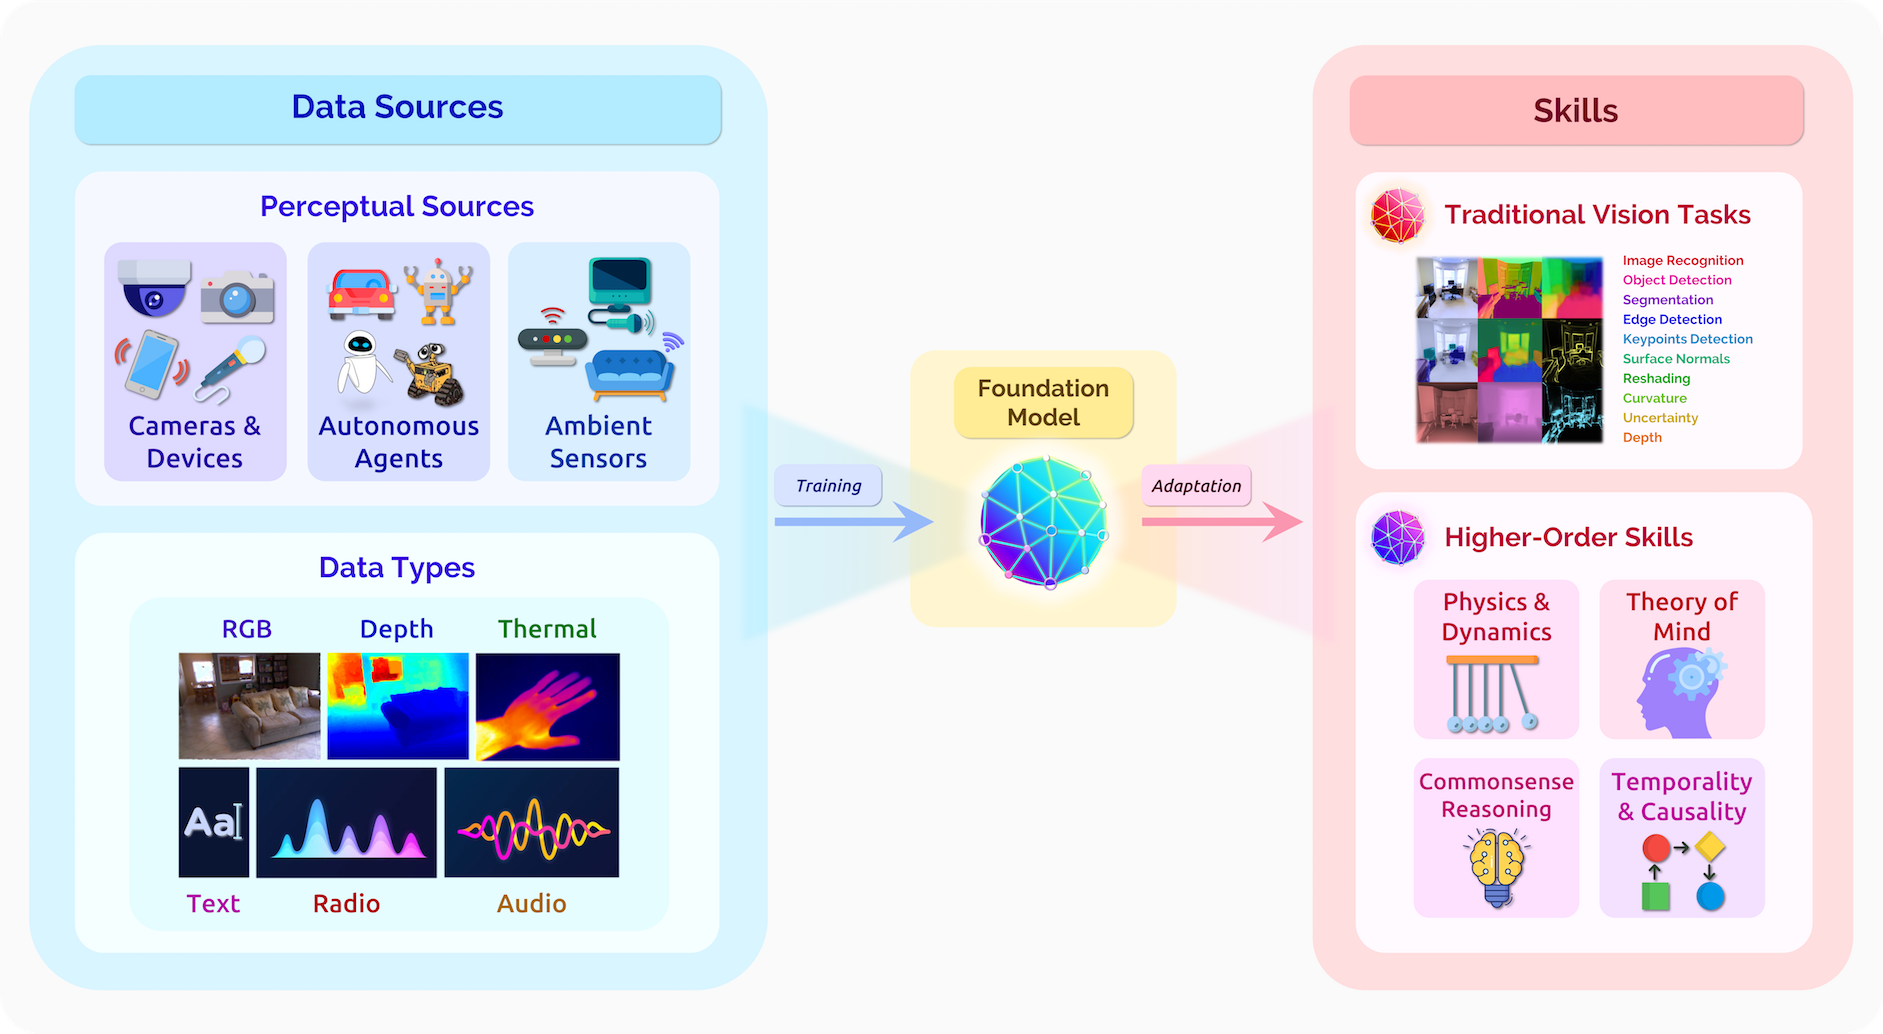
\includegraphics[width=\linewidth]{capabilities/figures/Vision.png}
% \vspace{-8mm}
\caption{\label{fig:vision}
By harnessing self-supervision at scale, foundation models for vision have the potential to distill raw, multimodal sensory information into visual knowledge, which may effectively support traditional perception tasks and possibly enable new progress on challenging higher-order skills like temporal and commonsense reasoning (\refsec{vision-capabilities}). These  inputs can come from a diverse range of data sources and application domains, suggesting promise for applications in healthcare and embodied, interactive perception settings (\refsec{vision-challenges}). Image credits \cite{zamir2018taskonomy, haque2020illuminating}.
}
\end{figure}

Vision underlies one of the primary modes through which a living organism understands its environment. 
The ability to see enables the near-constant, long-range gathering of dense signals, a capability so important that researchers have hypothesized that the development of eyes millions of years ago triggered a ``Cambrian explosion'' in evolution from which sprung many of the life forms we know today\dash{}among them, ourselves~\cite{parker2003blink}. 
For a skill executed effortlessly by even simple living creatures, transferring the same abilities to machines has proved remarkably challenging, leading computer vision and robotics researcher Hans Moravec in 1988 to observe a paradox: in AI, hard problems are easy and easy problems are hard, and among the ``easiest'' problems of them all is the visual acuity which we use each day to continually interpret complex scenes in a matter of milliseconds \cite{moravec1988mind,Thorpe1996,feifei2007we}.

On the other end of this formidable challenge is the substantial scope of transformative applications which computer vision holds the key to: self-driving cars that can free commuters from gridlock (\refsec{robotics}), life-saving AI tools that can assist overworked specialists by detecting rare medical events (\refsec{healthcare}), next-generation tools for multimedia creation and editing (\refsec{interaction}), among others. Reflecting on the applications and settings where human perception is fundamental offers a sense of the potential areas where computer vision can assist and transform.

The field of computer vision and the challenges we define draw inspiration in many ways from human perception capabilities.
Several classical theories \citep[\eg][]{biederman_perceiving_1972,mcclelland1981interactive,marr1982vision} suggested that humans may perceive real world scenes by contextualizing parts as a larger whole, and pointed the way for computer vision techniques to progressively model the physical world with growing levels of abstractions \cite{lowe1992robust,girshick2014rich}.
\citet{gibson1979ecological} suggested that human vision is inherently embodied and interactive ecological environments may play a key role in its development.
These ideas continue to motivate the ongoing development of computer vision systems, iterating towards a contextual, interactive, and embodied perception of the world.

In the context of computer vision, foundation models translate raw perceptual information from diverse sources and sensors into visual knowledge that may be adapted to a multitude of downstream settings (\reffig{vision}). To a large extent, this effort is a natural evolution of the key ideas that have emerged from the field over the last decade.
The introduction of ImageNet \cite{deng2009imagenet} and the advent of supervised pretraining led to a deep learning paradigm shift in computer vision. This transition marked a new era, where we moved beyond the classic approaches and task-specific feature engineering of earlier days \cite{lowe2004distinctive, bay2006surf, rosten2006machine} towards models that could be trained once over large amounts of data, and then adapted for a broad variety of tasks, such as image recognition, object detection, and image segmentation \cite{krizhevsky2012imagenet, szegedy2015going, he2016deep, simonyan2015verydeep}. This idea remains at the core of foundation models.

The bridge to foundation models comes from the limitations of the previous paradigm. Traditional supervised techniques rely on expensive and carefully-collected labels and annotations, limiting their robustness, generalization and applicability; in contrast, recent advances in self-supervised learning \cite{chen2020simclr, He2020MomentumCF}
suggest an alternative route for the development of foundation models that could make use of large quantities of raw data to attain a contextual understanding of the visual world. Relative to the broader aims of the field, the current capabilities of vision foundation models are currently early-stage (\refsec{vision-capabilities}): we have observed improvements in traditional computer vision tasks (particularly with respect to generalization capability) \cite{radford2021learning,ramesh2021zeroshot} and anticipate that the near-term progress will continue this trend. However, in the longer-term, the potential for foundation models to reduce dependence on explicit annotations may lead to progress on essential cognitive skills (\eg~commonsense reasoning) which have proven difficult in the current, fully-supervised paradigm \cite{zellers2019vcr,martin2021jrdb}.
In turn, we discuss the potential implications of foundation models for downstream applications, and the central challenges and frontiers that must be addressed moving forward (\refsec{vision-challenges}).


\subsubsection{Key capabilities and approaches}
\label{sec:vision-capabilities}

At a high-level, computer vision is the core sub-field of artificial intelligence that explores ways to endow machines with the capacity to interpret and understand the visual world. It encompasses a multitude of tasks, sub-domains and downstream applications, where the community has made continual progress over the last several decades \cite{zamir2018taskonomy}. A selection of example tasks\footnote{This, of course, is a coarse selection: please see the categories at the annual conference on Computer Vision and Pattern Recognition (CVPR) for a more complete (but evolving) picture of the tasks in the field.}:
(1) \textit{semantic understanding} tasks, which aim to discover the properties and relations among entities within visual scenes; these include image classification, object detection, semantic segmentation, action recognition, and scene graph generation, among others \citep[\eg][]{krizhevsky2012imagenet, he2016deep,  krishna2017visual, russakovsky2015imagenet, krizhevsky2009learning, kay2017kinetics, lin2014microsoft}. (2) \textit{geometric, motion and 3D} tasks, seeking to represent the geometry, pose and structure of still or moving objects, and include tasks of depth estimation, structure-from-motion, surface normal detection, curvature line and keypoint estimation, to name a few \citep[\eg][]{laina2016deeper, agarwal2011building, wang2015designing, zamir2018taskonomy, ullman1979interpretation}.
(3) \textit{multimodal integration} tasks, combining semantic and geometric understanding with other modalities such as natural language; these include, for instance, visual question answering, image captioning, and instruction following \citep[\eg][]{antol2015vqa, chen2015microsoft, anderson2018vision, goyal2017making, hudson2019gqa, johnson2017clevr, luo2020univl, akbari2021vatt, huang2021seeing, tsimpoukelli2021multimodal}. 
We highlight a subset of traditional core tasks in \reffig{vision}.

The predominant paradigm for addressing these tasks, driven by the emergence of ImageNet \cite{deng2009imagenet} during the early 2010s, tends to center around a familiar core idea:
First, pretrain a model on a large collection of carefully annotated data \cite{russakovsky2015imagenet} with a fully supervised training task, like image classification. Then, adapt the model downstream on task-specific datasets and domains \cite{lin2014microsoft, chen2015microsoft, antol2015vqa} by fine-tuning to reach state-of-the-art performance \cite{krizhevsky2012imagenet, simonyan2015verydeep, he2016deep, xu2016ask}.
This notion of pretraining followed by adaptation persists in the definitions we consider now for foundation models (\refsec{introduction}).
The limitations of this fully supervised paradigm motivate the transition to foundation models: the reliance on external supervised annotations constrains the upper bound capability of previous approaches to capture the diverse spectrum of visual inputs in a scalable, robust and generalizable manner. 
Recent developments in the domain of visual synthesis and unsupervised learning offer a compelling alternative. GANs, for instance, learn to generate visual content of high fidelity, realism and diversity, by featuring two competing networks of a generator and a discriminator that can supervise one another from image collections alone \citep[\eg][]{goodfellow2014gan,ganformer}. Other neural models infer the visual properties of objects and scenes without explicitly annotated supervision, by employing variational auto-encoding, contrastive learning or other self-supervised techniques \citep[\eg][]{Kingma2014AutoEncodingVB, chen2020simclr, He2020MomentumCF}.

With foundation models, the development of such self-supervision techniques has enabled training at greater scales of visual data \cite{changpinyo2021cc12m}, 
both in terms of its scope as well as its potential diversity. Accordingly, we have seen early indicators of progress on traditional vision tasks in terms of both standard accuracy metrics and few-shot generalization. For image classification and object detection, self-supervised techniques have reported competitive performance to prior fully-supervised approaches \cite{he2019moco,chen2020simclr,radford2021learning,henaff2021efficient}, without explicit annotations during training and greater sample efficiency during adaptation.
For visual synthesis, notable examples include DALL-E \cite{ramesh2021zeroshot} and CLIP-guided generation \cite{radford2021learning, galatolo2021generating}, where researchers leverage multimodal language and vision input to render compelling visual scenes.
In the short-term, we anticipate that the capabilities of these foundation models will continue to improve along these directions, as training objectives are refined \cite{chen2020mocov2,henaff2021efficient,selvaraju2021casting} and architectures are designed to incorporate additional modalities \cite{jaegle2021perceiver}.

Notably, current foundation models for computer vision are nascent relative to their NLP counterparts (\refsec{language}): promising early efforts are still largely centered on RGB image inputs and a subset of core traditional vision tasks. However, the field continues to progress on broader challenges centered on embodied and interactive perception settings (critical for foundation models for robotics, \refsec{robotics}). We note a subset of these higher-order goals in \reffig{vision}, including physical scene understanding, reasoning over visual commonsense and temporal events, and perception for social affordances.
Each of these have been goals for fully-supervised systems, but have proven challenging in part due to the difficulty of annotating these tasks at scale. 
For instance, standard systems for visual-question answering struggle to answer questions that require commonsense understanding, since these questions often require external knowledge beyond what is present in the pixels alone~\cite{zellers2019vcr}. Perceiving human gaze and social affordances in a robust manner remain ongoing challenges for embodied vision systems in interactive agents~\cite{martin2021jrdb}. By reducing the dependence on explicit annotations, foundation models may enable further progress towards these goals than was previously feasible. Related progress in language foundation models (\refsec{language}), which have been able to capture a degree of commonsense over language events \cite{brown2020gpt3}, also suggests a potential avenue towards achieving similar capability over multimodal visual inputs. While the exact roadmap for how to achieve these capabilities in foundation models remains an open problem, a combination of new efficient architectures (\refsec{modeling}), large-scale training (\refsec{systems}), self-supervision techniques (\refsec{training}) and few-shot adaptation schemes (\refsec{adaptation}) may open the door towards capabilities that have been difficult to reach so far.

\subsubsection{Central research challenges}
\label{sec:vision-challenges}

Our discussion of research challenges is motivated by the \textit{downstream application domains} where foundation models may further the integration and impact of vision models. 
We highlight a few such areas:
(1) \textit{ambient intelligence} for healthcare and home environments: building upon existing approaches for ambient intelligence in these settings \cite{haque2017towards, lyytinen2002ubiquitous, hong2004architecture}, foundation models may offer the potential for better detection of fine-grained human activities and medical events, as well as improved assistive interaction for clinicians, patients, and everyday consumers (see also \refsec{healthcare}).
(2) \textit{mobile and consumer applications}: foundation models with stronger multimodal grounding may enable more capable interactivity of services in mobile settings, and fundamental improvements in generation capability from vision and language inputs can benefit computational photography and content editing applications  \cite{delbracio2021mobile,ramesh2021zeroshot,park2019gaugan} (see also \refsec{interaction}).
(3) \textit{embodied, interactive agents}: perception models have already proven effective as both inputs  \cite{sermanet2018time} and reward functions  \cite{chen2021generalizable} in robotics settings; foundation models trained on large and/or simulated collections of egocentric visual data \cite{damen2018kitchens,chen2021geosim} may potentially further this progress by capturing a wider distribution of visual scenes, objects, and actions (see also \refsec{robotics}).

The extent to which foundation models may further impact these application settings hinges on the degree to which the capabilities outlined in \refsec{vision-capabilities} are realized. To bridge the significant gaps between present, short-term, and long-term anticipated capabilities, we must address current \textit{limitations} of foundation models for vision, including their training and evaluation. Below, a subset of corresponding key challenges:

\paragraph{Semantic systematicity and perceptual robustness.} Humans have a remarkable capacity for generalizing visual understanding to unseen compositions, and reasoning about the physical and geometric properties of novel objects and scenes \cite{lake2015human}. While current foundation models have shown promising capability for image synthesis and early results for generalization to fine-grained language inputs, these models still struggle to generalize to compositions of simple shapes and colors \cite{ramesh2021zeroshot,radford2021learning,rong2021extrapolating}. Generalizability goes beyond semantics as well; visual scenes and objects have a natural regularity to their physical dynamics and geometric properties. Foundation models have shown early indications of understanding scene and object geometry \cite{ramesh2021zeroshot}. Further, early efforts towards physical scene and geometric understanding in perception models may provide guidance for ongoing foundation model development \cite{yi2019clevrer, bakhtin2019phyre, li2020visual}. Indeed, the continued incorporation of multiple modalities (\eg~audio) in foundation models may prove beneficial towards these aims \cite{zhang2017shape,gao2020visualechoes,jaegle2021perceiverio}. However, the specific techniques to enable generalizing the initial observed capabilities robustly to a wide range of natural scenes and objects at the level of humans remains an open research challenge for foundation models.

\paragraph{Computational efficiency and dynamics modeling.} Humans are surprisingly efficient at processing the continuous visual stream of objects, scenes, and events necessary to support an understanding of event dynamics \cite{zacks2001perceiving, tversky2013event}.
Foundation models in language (\refsec{language}) have shown initial steps towards modeling longer-term coherence of events;
the analogous ability to capture long-range temporal correlations and causal coherence in visual input would stand to benefit downstream settings like robotics \citep[][\refsec{robotics}]{dai2019transformer,alyamkin2019low, goel2020survey,feng2019computer}.
However, relative to word token-level inputs in language, low-level computer vision inputs are extremely high-dimensional: a single 1080p frame contains over 2 million pixels. In this context, modeling the richer event dynamics in long-range video sequences seems like a daunting endeavor, especially with additional modalities (\eg~speech, optical flow, etc.) and increasing resolutions. Understandably, a na\"{i}ve approach to fully processing every individual pixel is likely prohibitive. Current vision models \citep[\eg][]{radford2021learning,sun2019videobert,tan2019lxmert,kim2021vilt} often address this by processing embeddings that summarize image patches or even groups of frames altogether, but this has the potential drawback of losing fine-grained details \cite{ramesh2021zeroshot}. In addition to considerations of the raw input space, foundation models for vision may need to revisit the design of fundamental architecture primitives (\refsec{modeling}) for efficient and effective modeling: alternatives to 3D convolutions may better address its cubic complexity \cite{fanbuch2020rubiks,sitzmann2019scene}, while particle-based representations may prove more effective for modeling physical dynamics \cite{bear2021physion}. Further, deployment of these vision models to downstream application settings will also necessitate advancements in systems design (\refsec{systems}). Taken together, the bottleneck of efficient and effective modeling for larger-scale, dynamic vision inputs remains a multi-faceted research direction that must be addressed going forward.

\paragraph{Training, environments, and evaluation.} Equally critical to realizing the potential of foundation models are the supporting elements for training and evaluating them. Current foundation models for vision have largely focused on a small subset of modalities shown in \reffig{vision} (\eg~datasets of RGB images and text), since these are perhaps the most readily accessible \cite{changpinyo2021cc12m,radford2021learning}. This motivates the development and use of additional large-scale training datasets which contain a diverse collection of inputs across a broad spectrum of modalities. While additional annotations may not strictly be necessary, the input quality impacts the learning efficiency of the models; techniques that leverage foundation models of other types (\eg~language) to help improve quality are a promising route forward \cite{zellers2021merlot}. 
We also want to consider settings beyond static datasets: classic studies have suggested that perceptual understanding in humans is linked to its embodiment and interactive, ecological settings \cite{gibson1979ecological}. As stepping stones towards longer-term capabilities of embodiment and interaction (\refsec{robotics}), ongoing development of simulation environments that capture physical, visual, and ecological realism with multiple modalities and viewpoints may play an important role in providing scalable and high-fidelity visual inputs for this goal \cite{kolve2017ai2thor,habitat19iccv,gan2020threedworld,shen2021igibson,srivastava2021behavior}. Finally, there is the question of metrics: how do we evaluate the faithfulness of generative foundation model outputs with respect to semantics? Standard metrics like Fr\'{e}chet Inception Distance, suffer from known flaws \cite{bikowski2018demystifying}; such issues parallel ones in natural language processing (\eg~metrics like BLEU do not correlate with causal judgements from humans). Having human judgements as part of evaluation may be one route, but incurs significant cost and may not be as scalable \cite{zhou2019hype,khashabi2021genie}. The outstanding and open challenges surrounding the training (\refsec{training}), data (\refsec{data}), and evaluation (\refsec{evaluation}) settings for vision foundation models are indeed quite nuanced, and will be a central area of research going forward.

\paragraph{Concluding remarks.} In this section, we explored foundation models in the context of computer vision, from identifying roots in previous computer vision paradigms, to contextualizing its current and anticipated capabilities, to proposing research directions moving forward. 
We conclude with a brief discussion of some broader \textit{societal implications} of foundation models for computer vision and their continued development (see also \refsec{society}).
The ubiquity of cameras in our society means that advances in computer vision techniques have great potential for disruptive impact; this carries a corresponding burden of responsibility for careful consideration of its risks. 
There is a well-documented history of learned bias in computer vision models, resulting in lower accuracies and correlated errors for underrepresented groups, with consequently inappropriate and premature deployment to some real-world settings \citep[\eg][\refsec{fairness}]{buolamwini2018gender}. 
Many of the same underlying issues continue to persist in current foundation models \cite{agarwal2021evaluating}. 
As data from additional sensor modalities (\eg~wearable or ambient sensors, \reffig{vision}) become incorporated in these foundation models, concerns surrounding privacy and surveillance become paramount (see \refsec{ethics}).
Furthermore, generated deepfake images and misinformation pose greater risks as the semantic and generative capability of vision foundation models continues to grow \citep[][\refsec{misuse}]{dolhansky2020deepfake,ramesh2021zeroshot}.
While the intriguing open challenges and opportunities ahead for computer vision and foundation models are significant, addressing these and related risks concurrently remains essential.